\chapter[Fundamental problem of risk prediction]{The fundamental problem of risk prediction for individuals: health AI, uncertainty, and personalized medicine}
% Only include if the thesis is written as a collection of papers
%_________________________
\label{sec:chp_FundamentalProblem}

\glsunset{AI}
\glsunset{ADNEX}
\glsunset{AUC}
\glsunset{IOTA}
\glsunset{RU}

\includegraphics*[width=0.3\linewidth]{logos/arxiv-logo.png}\vspace{0.5cm}

published as: 
\begin{quote}
Barreñada L, Steyerberg E, Timmerman D, Thomassen D, Wynants L, Van Calster B. The fundamental problem of risk prediction for individuals: health AI, uncertainty, and personalized medicine. npj Digital Medicine (submitted).
\end{quote}
\begin{quote}
\textbf{Supplementary material and code} available at \url{https://osf.io/2h9g5/}.
\end{quote}
\vspace{-0.5em}
\noindent\scriptsize\textit{Submitted for the first time: 09/05/2025 \quad Published: --- \quad APC: ---€}
\normalsize\vspace{-0.5em}
%_________________________
\section*{Summary}\label{abstract}

Clinical prediction models for a health condition are commonly evaluated regarding performance for a population, although decisions are made for individuals. The classic view relates uncertainty in risk estimates for individuals to sample size (estimation uncertainty). We show empirically that estimation uncertainty can be strongly dominated by model uncertainty (variability in modeling choices) and applicability uncertainty (variability in measurement procedures and between populations), even for models that perform well at the population level. Estimation uncertainty decreased considerably with increasing training sample size, whereas model and applicability uncertainty remained large. Hence, individual risk estimates are far more uncertain than often assumed. AI should inform, not dictate, care supporting personalization through clinician-patient interaction rather than through inherently uncertain model outputs. 

\newpage

\section{Introduction}

Clinical risk prediction models, which are increasingly based on artificial intelligence (AI), estimate the probability of a medical event occurring in a patient, conditional on a set of predictors \cite{steyerberg2019clinical}. Examples include models to estimate the 10-year risk of coronary heart disease \cite{hippisley-coxDevelopmentValidationQRISK32017}, early mortality in cardiac surgical patients \cite{nashefEuroSCOREII2012}, the risk of ovarian cancer \cite{vancalsterEvaluatingRiskOvarian2014}, the 10-year mortality risk of breast cancer patients \cite{candidodosreisUpdatedPREDICTBreast2017}, or the risk of deterioration in hospitalized patients with COVID \cite{guptaDevelopmentValidationISARIC2021}.

The performance of prediction models is usually assessed at the population level. To make informed decisions for an individual patient, however, the focus is on the risk estimates for that individual. The trustworthiness of individual risk estimates is commonly ignored in practice, and rarely evaluated or quantified \cite{altmanWhatWeMean2000}. We aim to present a structured framework of the key sources of uncertainty in risk estimation for individuals, and to expose the magnitude of uncertainty arising from sources that are typically hidden in practice. We illustrate this with a case study on estimating the risk of cancer in patients presenting with an ovarian tumor.

\section{A framework for uncertainty}

Uncertainty and the concept of `individual risk' have been studied for centuries \cite{sternAccuracyPreoperativeRisk2025,altmanWhatWeMean2000,hackingEmergenceProbabilityPhilosophical2006,finettiTheoryProbabilityCritical1979,vennLogicChance1876,vonmisesProbabilityStatisticsTruth1957,laplacePhilosophicalEssayProbabilities1902,lemeshowOutcomePredictionIndividual1995,hendersonIndividualSurvivalTime2005,steyerbergEquallyValidModels2005}. An individuals' risk of an event as estimated by a prediction model refers to the probability of that event in the subgroup of individuals with the same predictor values. Truly individual risks do not exist because of the `reference class problem': an individual can belong to an infinite number of subgroups. By choosing a different set of predictors to condition on, the reference class changes, and so does the risk. Yet, despite the philosophical challenges in defining a true individual risk, risk estimates are routinely used in practice, making it crucial to understand the different types of uncertainty they carry. For predictive modeling, a basic decomposition of uncertainty is into aleatoric and epistemic uncertainty (Table~\ref{tab:5:1} and Figure~\ref{fig:5:1}) \cite{hullermeierAleatoricEpistemicUncertainty2021,sengeReliableClassificationLearning2014}. Aleatoric uncertainty refers to the inherent random nature of the event we want to predict. Two patients who have the same values for the predictors in the best possible model may still have a different outcome. This does not invalidate the prediction. In contrast, epistemic uncertainty refers to lack of knowledge about the best possible model. We break down epistemic uncertainty for predictive modeling into three key categories: estimation, model, and applicability uncertainty (Table~\ref{tab:5:1}).


\begin{table}
\centering
\small
\caption[Overview of epistemic uncertainty]{Overview of the categories of epistemic uncertainty.}
\label{tab:5:1}
\begin{tabularx}{\textwidth}{>{\raggedright\arraybackslash}p{0.25\textwidth} >{\raggedright\arraybackslash}X >{\raggedright\arraybackslash}X}
  \toprule
  \textbf{Description} & \textbf{Examples} & \textbf{Actions} \\
\midrule
	\textbf{ESTIMATION UNCERTAINTY} & Instability of the fitted model due to finite training sample size. If we collect two datasets from the same population with the same sample size and sampling procedures, and train the same model on both datasets, the estimated model parameters will differ. & Increase sample size; quantify instability (e.g. 95\% confidence intervals or effective sample size) \cite{thomassenEffectiveSampleSize2024}. \\
\addlinespace
	\textbf{MODEL UNCERTAINTY} & Uncertainty due to lack of knowledge about the optimal model specification (model class, feature specification, transformations, selection, hyperparameter tuning). & Improve education about good modeling practice; conduct literature searches and exploratory studies; run pilot comparisons of model classes. \\
\addlinespace
	\textbf{APPLICABILITY UNCERTAINTY (DATA)} & Variability in data collection procedures: differing variable definitions, measurement methods, assay kits, inter-rater variability, and missing-data mechanisms \cite{luijkenImpactPredictorMeasurement2019,agnielBiasesElectronicHealth2018}. & Standardize definitions and measurement procedures; empirically compare measurement methods; invest in data cleaning, linkage, and harmonization. \\
\addlinespace
	\textbf{APPLICABILITY UNCERTAINTY (POPULATIONS)} & Variability between populations in case-mix, prevalence, treatment pathways, and associations between predictors and outcome; population drift over time \cite{davisCalibrationDriftRegression2017}. & Conduct multicenter studies; quantify heterogeneity (leave-center-out CV, meta-analysis with prediction intervals); consider local validation and updating \cite{swaminathanReflexiveRecalibrationCausal2025}. \\
\bottomrule
\end{tabularx}
\end{table}


\begin{figure}
\centering
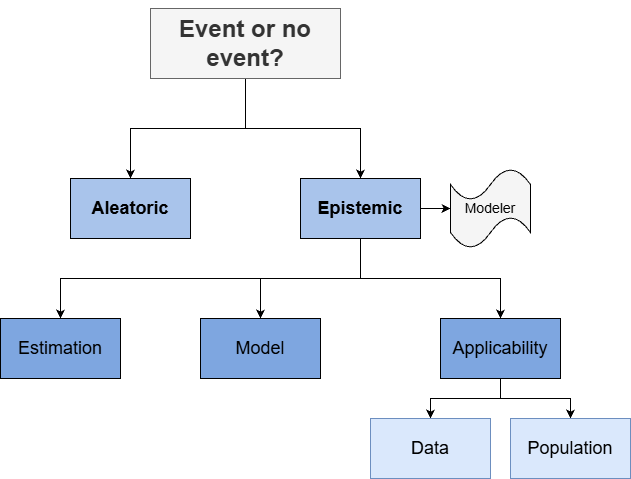
\includegraphics[width=0.9\textwidth]{figures/FundamentalProblem/F1.png}
\caption[A framework of uncertainty when predicting risk for the individuals]{A framework of uncertainty when predicting risk for the individuals.}
\end{figure}



We evaluated population-level performance using the \gls{AUROC} for discrimination, \gls{ECI} for calibration (\gls{ECI}=0 means perfect calibration), and relative utility (\gls{RU}) for clinical utility (\gls{RU}$\leq$0 means no utility) \cite{vanhoordeAssessingCalibrationMultinomial2014,bakerUsingRelativeUtility2009}. To evaluate individual-level variability, we calculated for each patient the 95\% range and \gls{DU} of 59,400 estimated risks per sample size. The 95\% range is the estimated risk at the 97.5th percentile minus the estimated risk at the 2.5th percentile. \gls{DU} is lowest of the proportions of models that yield an estimated risk \textless0.1 vs $\geq$0.1. This is a common threshold in this setting \cite{timmermanESGOISUOGIOTA2021}. If all models yield a risk on the same side of the threshold, there is no \gls{DU} (\gls{DU}=0). If half of the models yield a risk above the threshold, and half below, there is maximal uncertainty (\gls{DU}=0.5). See Appendix 1 in online methods for details.

\section{Results}

\subsection{Estimation uncertainty}

Consider the estimated risk of ovarian cancer for 100 new patients (i.e. patients whose data was not used in model building) according to 100 identical models, each fitted on a different random sample from one population. For some patients, the risk estimates (on a scale from 0 to 1) varied considerably, particularly at small training sample sizes (Figure~\ref{fig:5:2}, left). The mean 95\% range of estimated risks for a new patient decreased from 0.22 for training sets with N=400 to 0.04 for training sets with N=10,000 (Table~\ref{tab:5:2}). When a risk estimate of 0.1 or higher was used as the threshold to recommend surgery for a single new patient, on average 6\% of models trained on a dataset of 400 patients would suggest a different decision than the majority of models. Increasing the training set to 10,000 patients reduced this decision uncertainty to 1\%. We observed that estimation uncertainty is higher and decreases more slowly with increasing training sample size for tree-based models compared to logistic regression (Table~\ref{tab:5:2} and Table S3, Supplementary Figure S3). In contrast to the indicators of uncertainty at the individual level, the population level discrimination and calibration remained rather stable across training sample sizes. The positive population level \gls{RU} indicates the model is useful to support clinical decision-making at all sample sizes.

\begin{table}
\centering
\footnotesize
\caption[Population level performance and individual risk uncertainty]{Population level performance and individual risk uncertainty for the 100 test set patients.}
\label{tab:5:2}
\resizebox{\textwidth}{!}{
\begin{tabular}{l l c c c c c}
\toprule
 &  & \multicolumn{3}{c}{\textbf{Population level performance}} & \multicolumn{2}{c}{\textbf{Individual level uncertainty}} \\
 \midrule

\multirow[c]{2}{*}{\textbf{Source}} & \multirow[c]{2}{*}{\textbf{Training data}} & \textbf{AUROC} & \textbf{ECI} & \textbf{RU} & \textbf{95\% range} & \textbf{DU} \\
&  & \textit{mean (range)} & \textit{mean (range)} & \textit{median$^a$ (range)} & \textit{mean (range)} & \textit{mean (range)} \\
\midrule
\multirow[c]{3}{*}{Estimation} & 400 & .92~(.89;~.93) & .11~(.02;~.21) & .05~(-.61;~.49) & .22~(.01;~.65) & .06~(0;~.49) \\
& 2000 & .92~(.91;~.93) & .11~(.06;~.14) & .20~(-.02;~.49) & .10~(.01;~.36) & .02~(0;~.33) \\
& 10000 & .93~(.92;~.93) & .11~(.10;~.13) & .18~(.02;~.37) & .04~(.00;~.14) & .01~(0;~.31) \\
\addlinespace
\multirow[c]{3}{*}{All sources} & 400 & .92~(.79;~.98) & .11~($<$.01;~.93) & .16~(-2.2;~.82) & .46~(.07;~.91) & .12~(0;~.50) \\
& 2000 & .93~(.84;~.98) & .10~($<$.01;~.68) & .18~(-2.0;~.82) & .41~(.06;~.95) & .11~(0;~.50) \\
& 10000 & .93~(.83;~.98) & .09~($<$.01;~.55) & .18~(-1.5;~.84) & .39~(.06;~.98) & .11~(0;~.50) \\
\bottomrule
\end{tabular}
}
\begin{minipage}{\textwidth}
\vspace{0.5em}
\scriptsize
AUROC: Area under the receiver operating characteristic curve; AUROC 0.5 indicates that the model cannot discriminate between patients with and without ovarian cancer, AUROC 1 indicates perfect discrimination. ECI: Estimated calibration index; ECI is scaled between 0 and 1 with 0 indicating that estimated risks correctly estimate risk at the population level. RU: Relative utility; RU can take on values between $-\infty$ and 1 where positive values indicate the model has clinical utility to support decision making and values $\leq$ 0 indicate that the model has no clinical utility. 95\% range: range of the middle 95\% of risk estimates across all models for one individual; 0 indicates no uncertainty, 1 indicates maximal uncertainty. DU: Decision uncertainty for an individual when using the model at a threshold of 0.1 on the risk of malignancy to suggest a management decision. DU ranges between 0 and 0.5, with 0 indicating that all models suggest the same decision, and 0.5 that half of the models suggest to operate and the other half suggest conservative management.

\textsuperscript{a} We used median because negative values for RU can be very low and distort the results.
\end{minipage}
\end{table}

\begin{figure}
\centering

\includegraphics[width=0.9\textwidth]{figures/FundamentalProblem/F2.png}
\caption[Uncertainty in estimated risks for individual patients]{Visualization of the uncertainty in the estimated risks for individual patients. Panels on the left show estimation uncertainty for the main model based on training sample sizes of 400 (top), 2000 (middle) and 10000 (bottom). Each panel contains the individual estimated risks (y-axis) for 100 test patients (x-axis) by 100 models based on randomly selected training datasets. The main model used unpenalized logistic regression with restricted cubic splines, with regression imputation for missing CA125, no variable selection, using training data from Leuven and with lesion size measured using the maximal diameter. Panels on the right show the total uncertainty for all 59,400 models. Each panel contains the individual estimated risks (y-axis) for 100 patients (x-axis) by 59,400 models based on combinations of modeling strategies, data properties, populations included at training (Supplementary Table S1) and on randomly selected training datasets. This means that each of the 100 patients has 59,400 predicted estimated risks.}
\label{fig:5:2}
\end{figure}

\subsection{Model and applicability uncertainty}

When also acknowledging model and applicability uncertainty, the differences in estimated ovarian cancer risks for any single patient from a total of 59,400 models were considerably larger than when acknowledging estimation uncertainty alone (Figure~\ref{fig:5:2}, right). Even when the training sample size was 10,000, the 95\% range in risk estimates for a single patient was on average 0.39 (range 0.05 to 0.99). The highest 95\% risk range for a single patient was 0.99, nearly covering all possible risk estimates between 0 and 1.

In contrast to approximation uncertainty, increasing the training sample size led to minimal reductions in model uncertainty and applicability uncertainty. On average, 12\% of models trained on 400 patients would lead to a different clinical decision for a single patient than most models suggest. When training was done on data of 10,000 patients, the decision uncertainty was still 11\%. Note that this is substantial compared to the maximum decision uncertainty of 50\% (when 50\% of models suggest to operate and 50\% of models suggest not to operate). Findings were similar for any class of models (Supplementary Table S3).

The mean \gls{AUROC} (0.92-0.93) and \gls{ECI} (0.09-0.11) values were similar to the values observed when we only considered estimation uncertainty (Table~\ref{tab:5:2}). Detailed results about estimation, model and applicability uncertainty available in Online Methods (Synthetic data: Supplementary Figures S3-S6; real data: Supplementary Figures S7-S10 and Supplementary Tables S4-S5).

\section{Discussion}

Precision medicine aims to target interventions towards the specific characteristics of the individual. In this context, prediction models and \gls{AI} algorithms can be valuable to improve decision making. Our study shows that, even though prediction models may perform very well at the population level (high discrimination, good calibration and clinical utility to support decisions), the uncertainty in estimated risks and suggested decisions for a single patient is often uncomfortably large.

Calibration assesses whether estimated risks correspond to observed proportions for (sub)groups of patients, typically using calibration metrics and plots, but does not inform on the uncertainty of risk estimates for an individual patient. The classic approach towards uncertainty assessment for an individual involves confidence intervals or other quantifications of variability that assume that modeling, data, and population decisions are fixed (estimation uncertainty, Table~\ref{tab:5:1}) \cite{rileyStabilityClinicalPrediction2023,thomassenEffectiveSampleSize2024,kompaSecondOpinionNeeded2021}. Recent research on clinical prediction models has focused on estimation uncertainty, i.e. instability as a function of sample size \cite{rileyStabilityClinicalPrediction2023,rileyClinicalPredictionModels2023,rileyUncertaintyRiskEstimates2025}. We demonstrated that the magnitude of model uncertainty and applicability uncertainty may extend far beyond estimation uncertainty. Estimation uncertainty differs from other sources of epistemic uncertainty in two aspects. First, it reduces more strongly with increasing sample size than other sources of uncertainty. Second, it can be visualized and quantified, whereas other sources are mostly invisible and hardly quantifiable. A few studies highlighted that modeling choices including model class, predictors, and missing data imputation techniques may impact on individual risk estimates \cite{ledgerMulticlassRiskModels2023,pateUncertaintyUsingRisk2019,liConsistencyVarietyMachine2020}. In the current analyses, we quantified how data-related choices (in measurement, definition and populations) further impact uncertainty. The number of decisions that are taken to develop a model is potentially infinite, yet we usually only see one specific model.

It may seem paradoxical that using prediction models for decision making can benefit outcomes at a population level without having trustworthy risk estimates for individuals from that population. This may cause skepticism about the acceptability of data-driven clinical decision support tools, either based on classical regression approaches or novel \gls{AI} algorithms. We argue that such skepticism is not needed. Clinical utility at the population level, for example in terms of cost-effectiveness, is sufficient to warrant the use of a decision strategy based on a model. We may need to accept that two models may have the same clinical utility yet very different risk estimates for the same individual, often to the extent that model A recommends treatment initiation, but model B does not. The enormous uncertainty on the individual level does have consequences. First, the uncertainty should be acknowledged and considered when discussing risks and treatment options with patients. Given the considerable impact of poorly quantifiable model and applicability uncertainty, further research is needed on how to integrate model predictions in the shared decision making process. Second, while we should strive to reduce epistemic uncertainty in clinical prediction models, we must also recognize and accept it as an unavoidable element of medical decision-making. Finally, we should be humble regarding the promises of personalized medicine \cite{sennStatisticalPitfallsPersonalized2018}. Health \gls{AI} will always provide highly uncertain group level estimations based on their training data, even if the group is defined very narrowly. As a consequence, the estimated risk for the individual is not personalized, yet the shared decision making based on this estimation can be.

Researchers have a variety of tools at their disposal to reduce or embrace epistemic uncertainty, listed in Table~\ref{tab:5:1}. First, to reduce estimation uncertainty, we need to develop models on sufficiently large sample sizes \cite{tsegayeLargerSampleSizes2025}. Whereas there are elegant sample size calculation procedures for prediction models based on regression, such procedures are lacking for machine learning algorithms, which may generally require large sample size to allow for flexible modeling \cite{rileyCalculatingSampleSize2020,vanderploegModernModellingTechniques2014}. Further, methods that allow prediction abstention due to uncertainty have been proposed \cite{kompaSecondOpinionNeeded2021,myersIdentifyingUnreliablePredictions2020}. Even though not all sources of uncertainty are included, it may be a good start to abstain from predictions based merely on estimation uncertainty, for example requiring at least an effective sample size of 10 patients per prediction \cite{rileyUncertaintyRiskEstimates2025,thomassenEffectiveSampleSize2024}. Second, a better agreement and education about good prediction modeling practices could reduce model uncertainty, including the effects of modeler uncertainty, to some degree. Third, to reduce data uncertainty, the use of prospective study designs can help. Retrospective studies tend to have increased uncertainty regarding the definition, measurement procedure, and availability of relevant predictors and outcome variables. Prospective studies, including randomized controlled trials, typically allow for better standardization of definitions and measurement protocols \cite{steyerbergPrognosisResearchStrategy2013}. For example, a set of `terms and definitions' has become standard in the field of ovarian tumors \cite{timmermanTermsDefinitionsMeasurements2000} and `common data elements' have been defined for traumatic brain injury studies \cite{maasOpportunitiesChallengesHighQuality2022,maasStandardizingDataCollection2011}. While sample size is important for model development, data quality should be prioritized over quantity for clinical prediction model development. Although a huge dataset further reduces estimation uncertainty, it may increase data uncertainty due to data quality problems. Fourth, population uncertainty may be exposed by assessing population differences and performance heterogeneity across sites in multicenter development and validation studies \cite{vancalsterThereNoSuch2023}. Monitoring and updating of prediction models can improve local performance and further decrease uncertainty. Ideally, this includes assessing the causes of the heterogeneity and performance changes over time \cite{youssefExternalValidationAI2023,swaminathanReflexiveRecalibrationCausal2025}.

The strength of our demonstration on ovarian cancer diagnostic modeling is the extensive investigation of different types of uncertainty on empirical data, and its presentation in easy-to-interpret metrics and simple visualizations. At the same time, this approach has a few limitations. First, we were constrained by the available data in our choices related to data and population uncertainty, likely leading to an underestimation of applicability uncertainty. Second, to investigate the results for models built on large training datasets, we created a larger synthetic dataset with identical properties as the original dataset. Third, the event of interest in our dataset was relatively common (37\% of tumors were malignant), which yields larger values for the 95\% range compared to situations where the event is rare. Of note, smaller 95\% ranges in cases with rare events may still affect decision uncertainty, if the decision threshold falls around instable predictions. Fourth, diagnostic models for ovarian malignancy have high \gls{AUROC} values (above 0.9). While higher levels of uncertainty might be present for prediction problems with lower discrimination, the amount of individual risk uncertainty is striking for a model that is well able to distinguish between patients with the event and patients without it at the population level. Finally, although we considered a large number (594) of scenarios, more scenarios could have been conceived. For example, we did not vary the set of six predictors, and our variations in the tree-based algorithms were less extensive than those for the logistic regression analysis. These characteristics of the data and selected scenarios enforce the conclusions of our study, given that most of these issues have most likely underestimated the full uncertainty.

In conclusion, a fundamental problem in risk prediction is that individual risk estimates may be highly uncertain, even for models with high discriminatory ability that improve outcomes for the population when used to guide decision making. The uncertainty for predictions at the individual level will often be considerably larger than suggested by classic uncertainty measures such as 95\% confidence intervals or novel measures such as effective sample size \cite{thomassenEffectiveSampleSize2024}. This uncertainty does not invalidate the clinical utility of well-developed prediction models at a population level, but urges great caution when interpreting and discussing risk estimates with individual patients in clinical practice.



\subsection*{Funding} This research is supported by Research Foundation -- Flanders (FWO) grants G097322N, G049312N, G0B4716N, and 12F3114N to BVC and/or DTi, KU Leuven internal grants C24M/20/064 and C24/15/037 to BVC and/or DTi, ZoNMW VIDI grant 09150172310023 to LW. DTi is a senior clinical investigator of FWO. No funding source had any role in the study design, data collection,data analysis, data interpretation, writing, or submission of this report.

\subsection*{Author contributions} Conceptualization: BVC. Methodology: LB, ES, LW, DTh, BVC. Investigation: LB, BVC. Visualization: LB, BVC. Funding acquisition: DTi, LW, BVC. Project administration: LB. Supervision: ES, BVC. Writing -- original draft: LB, LW, BVC. Writing -- review \& editing: LB, ES, DTi, DTh, LW, BVC.

\subsection*{Competing interests} Authors declare that they have no competing interests.

\subsection*{Data and materials availability} Synthetic and real data are not publicly available, but we provide the individual risk estimations of all the different models and explanatory code to reproduce all the results in this work in the OSF repository (https://osf.io/uxvhq/)
